\documentclass{beamer}
\usepackage[utf8]{inputenc}
\usepackage{graphicx, epsfig}
\usepackage{amsmath,mathrsfs,amsfonts,amssymb}
\usepackage{floatflt}
\usepackage{epic,ecltree}
\usepackage{mathtext}
\usepackage{fancybox}
\usepackage{fancyhdr}
\usepackage{multirow}
\usepackage{enumerate}
\usepackage{epstopdf}
\usepackage{multicol}
\usepackage{algorithm}
\usepackage[noend]{algorithmic}
\usepackage{tikz}
\usepackage{blindtext}
\usepackage{multido}
\usetheme{default}%{Singapore}%{Warsaw}%{Warsaw}%{Darmstadt}
\usecolortheme{default}

\setbeamerfont{title}{size=\Huge}
\setbeamertemplate{footline}[frame number]{}

\setbeamertemplate{section in toc}[sections numbered]

\makeatletter
\newcommand\HUGE{\@setfontsize\Huge{35}{40}}
\makeatother    

\setbeamerfont{title}{size=\HUGE}
\beamertemplatenavigationsymbolsempty

\usetikzlibrary{arrows,shapes,positioning,shadows,trees}

\newcommand\myfootnote[1]{%
  \vspace{-0.5cm}%
  \tikz[remember picture,overlay]
  \draw (current page.south west) +(1in + \oddsidemargin,0.5em)
  node[anchor=south west,inner sep=0pt]{\parbox{\textwidth}{%
      \rlap{\rule{10em}{0.4pt}}\raggedright\scriptsize \textit{#1}}};}

\newcommand\myfootnotewithlink[2]{%
  \vspace{-0.5cm}%
  \tikz[remember picture,overlay]
  \draw (current page.south west) +(1in + \oddsidemargin,0.5em)
  node[anchor=south west,inner sep=0pt]{\parbox{\textwidth}{%
      \rlap{\rule{10em}{0.4pt}}\raggedright\scriptsize\href{#1}{\textit{#2}}}};}

\AtBeginSection[]
      {
      	\begin{frame}{Outline}
      		\tableofcontents[currentsection]
      	\end{frame}
      }
      \AtBeginSubsection[]{
      	\begin{frame}{Outline}
      		\tableofcontents[currentsection,currentsubsection]
      	\end{frame}
}

\newcounter{noscounter} % Используется для nextonslide команды (обнуляется только на новом слайде)
\newcounter{pcounter} % Используется для pause команды (обнуляется после использования eqpause)
\newcounter{diffcounter} % Считает количество pause после формулы

\newcommand{\nextonslide}[1]{%
  \stepcounter{noscounter}% Прибавляем счетчик nextonslide
  \stepcounter{pcounter}% Прибавляем счетчик pause
  \stepcounter{diffcounter}% Прибавляем счетчик diffcounter
  \onslide<\value{noscounter}->{#1}% Отображаем аргумент в скобках на слайде с номером noscounter
}
\newcommand{\resetonslide}{%
    \setcounter{noscounter}{1}% Сбрасываем счетчик nextonslide
    \setcounter{pcounter}{1}% Сбрасываем счетчик pause
    \setcounter{diffcounter}{0}% Сбрасываем счетчик diffcounter
}

\newcommand{\eqpause}{%
  \multido{\i=1+1}{\value{pcounter}}{\pause}% Повторяем pcounter раз команду pause
  \stepcounter{noscounter}% Прибавляем счетчик nextonslide
  \setcounter{pcounter}{1}% Сбрасываем счетчик pause
}

\newcommand{\eqpausediff}{% Вспомогательная команда, запускается автоматически после формул
  \multido{\i=1+1}{\value{diffcounter}}{\pause}% Повторяем diffcounter раз команду pause
  \addtocounter{pcounter}{-\value{diffcounter}}% Вычитаем из pcounter количество сделанных pause
  \setcounter{diffcounter}{0}% Сбрасываем счетчик diffcounter
}

\newcommand\AtEndBoth[2]{% Применяем команду к multline и multline*
  \AtEndEnvironment{#1}{#2}%
  \AtEndEnvironment{#1*}{#2}%
}

\AtEndBoth{align}{\eqpausediff}
\AtEndBoth{equation}{\eqpausediff}
\AtEndBoth{multline}{\eqpausediff}

\addtobeamertemplate{frametitle}{\resetonslide}{}% На каждом слайде сбрасываем счетчики

% latin bold lower
\newcommand{\ba}{\mathbf{a}} 
\newcommand{\bc}{\mathbf{c}} 
\newcommand{\be}{\mathbf{e}} 
\newcommand{\bff}{\mathbf{f}} % \bf - for bold type
\newcommand{\bg}{\mathbf{g}} 
\newcommand{\bh}{\mathbf{h}} 
\newcommand{\bp}{\mathbf{p}} 
\newcommand{\bq}{\mathbf{q}} 
\newcommand{\bt}{\mathbf{t}} 
\newcommand{\bs}{\mathbf{s}} 
\newcommand{\bu}{\mathbf{u}} 
\newcommand{\bv}{\mathbf{v}} 
\newcommand{\bw}{\mathbf{w}} 
\newcommand{\bx}{\mathbf{x}} 
\newcommand{\by}{\mathbf{y}} 
\newcommand{\bz}{\mathbf{z}} 

% latin bold upper
\newcommand{\bA}{\mathbf{A}} 
\newcommand{\bB}{\mathbf{B}} 
\newcommand{\bC}{\mathbf{C}} 
\newcommand{\bG}{\mathbf{G}} 
\newcommand{\bI}{\mathbf{I}} 
\newcommand{\bJ}{\mathbf{J}} 
\newcommand{\bL}{\mathbf{L}} 
\newcommand{\bM}{\mathbf{M}} 
\newcommand{\bP}{\mathbf{P}}
\newcommand{\bQ}{\mathbf{Q}} 
\newcommand{\bR}{\mathbf{R}} 
\newcommand{\bT}{\mathbf{T}} 
\newcommand{\bU}{\mathbf{U}} 
\newcommand{\bV}{\mathbf{V}} 
\newcommand{\bW}{\mathbf{W}} 
\newcommand{\bX}{\mathbf{X}} 
\newcommand{\bY}{\mathbf{Y}} 
\newcommand{\bZ}{\mathbf{Z}} 

% latin cal upper
\newcommand{\cF}{\mathcal{F}} 
\newcommand{\cG}{\mathcal{G}} 
\newcommand{\cI}{\mathcal{I}} 
\newcommand{\cL}{\mathcal{L}} 
\newcommand{\cM}{\mathcal{M}} 
\newcommand{\cN}{\mathcal{N}} 
\newcommand{\cP}{\mathcal{P}} 
\newcommand{\cS}{\mathcal{S}} 
\newcommand{\cT}{\mathcal{T}} 
\newcommand{\cW}{\mathcal{W}} 
\newcommand{\cX}{\mathcal{X}} 
\newcommand{\cZ}{\mathcal{Z}} 

% latin bb upper
\newcommand{\bbE}{\mathbb{E}} 
\newcommand{\bbI}{\mathbb{I}} 
\newcommand{\bbP}{\mathbb{P}} 
\newcommand{\bbR}{\mathbb{R}} 

% greek bold lower
\newcommand{\bepsilon}{\boldsymbol{\epsilon}} 
\newcommand{\btheta}{\boldsymbol{\theta}} 
\newcommand{\blambda}{\boldsymbol{\lambda}} 
\newcommand{\bpi}{\boldsymbol{\pi}} 
\newcommand{\bmu}{\boldsymbol{\mu}} 
\newcommand{\bsigma}{\boldsymbol{\sigma}} 
\newcommand{\bphi}{\boldsymbol{\phi}} 

% greek bold upper
\newcommand{\bSigma}{\boldsymbol{\Sigma}} 

\DeclareMathOperator*{\argmin}{arg\,min}
\DeclareMathOperator*{\argmax}{arg\,max}
\newcommand{\createdgmtitle}[1]{\title[\hbox to 56mm{Deep Generative Models  \hfill\insertframenumber\,/\,\inserttotalframenumber}]
	{\vspace{1cm} \\ \textbf{Deep Generative Models} \\ {\Huge Lecture #1}}
	\author{Roman Isachenko}
	\institute{
		Moscow Institute of Physics and Technology \\
		Yandex School of Data Analysis
	}
	\date{2025, Autumn}
}
\createdgmtitle{2}

%--------------------------------------------------------------------------------
\begin{document}
%--------------------------------------------------------------------------------
\begin{frame}[noframenumbering,plain]
\titlepage
\resetonslide
\end{frame}
%======
\begin{frame}{Recap of Previous Lecture}
	We're given \textbf{finite} number of i.i.d.\ samples $\{\bx_i\}_{i=1}^n \subset \bbR^m$ drawn from an \textbf{unknown} distribution $\pd(\bx)$.
	\begin{block}{Objective}
		Our aim is to learn a distribution $\pd(\bx)$ that allows us to: 
		\begin{itemize}
		    \item Generate new samples from $\pd(\bx)$ (sample $\bx \sim \pd(\bx)$) --- \textbf{generation}.		    
		    \item Evaluate $\pd(\bx)$ on novel data (answering ``How likely is an object $\bx$?'') --- \textbf{density estimation}; 
		\end{itemize}
	\end{block}

	\begin{block}{Divergence Minimization Task}
		\begin{itemize}
			\item $D(\pi \| p) \geq 0$ for all $\pi, p \in \cP$;
			\item $D(\pi \| p) = 0$ if and only if $\pi \equiv p$.
		\end{itemize}
		\[
		\min_{\btheta} D(\pd \| \pt)
		\]
	\end{block}
\end{frame}
%=======
\begin{frame}{Recap of Previous Lecture}
	\begin{block}{Forward KL Divergence}
		\vspace{-0.2cm}
		\[
		\KL(\pd \| \pt) = \int \pi (\bx) \log \frac{\pd(\bx)}{\pt(\bx)}\, d \bx \rightarrow \min_{\btheta}
		\]
	\end{block}
	\begin{block}{Reverse KL Divergence}
		\vspace{-0.2cm}
		\[
		\KL(\pt \| \pd) = \int \pt(\bx) \log \frac{\pt(\bx)}{\pd(\bx)}\, d \bx \rightarrow \min_{\btheta}
		\]
	\end{block}
	
	\begin{block}{Maximum Likelihood Estimation (MLE)}
		\vspace{-0.3cm}
		\[
		\btheta^* = \argmax_{\btheta} \prod_{i=1}^n \pt(\bx_i) = \argmax_{\btheta} \sum_{i=1}^n \log \pt(\bx_i)
		\]
		\vspace{-0.1cm}
	\end{block}
	Maximum likelihood estimation is equivalent to minimizing the Monte Carlo estimate of the forward KL divergence.
\end{frame}
%=======
\begin{frame}{Recap of Previous Lecture}
	\begin{block}{Likelihood as Product of Conditionals}
		Let $\bx = (x_1, \dots, x_m)$, and define $\bx_{1:j} = (x_1, \dots, x_j)$. Then,
		\[
		\pt(\bx) = \prod_{j=1}^m \pt(x_j | \bx_{1:j-1}), \quad 
		\log \pt(\bx) = \sum_{j=1}^m \log \pt(x_j | \bx_{1:j-1})
		\]
	\end{block}
	\vspace{-0.3cm}
	\begin{block}{MLE for Autoregressive Models}
		\vspace{-0.3cm}
		\[
		\btheta^* = \argmax_{\btheta} \sum_{i=1}^n \sum_{j=1}^m \log \pt(x_{ij} | \bx_{i, 1:j-1})
		\]
		\vspace{-0.5cm}
	\end{block}
	\begin{block}{Sampling}
		\vspace{-0.5cm}
		\[
		{\color{teal} \hat{x}_1} \sim \pt(x_1), \quad \hat{x}_2 \sim \pt(x_2 | {\color{teal} \hat{x}_1}), \quad \ldots, \quad \hat{x}_m \sim \pt(x_m | \hat{\bx}_{1:m-1})
		\]
		The generated sample is $\hat{\bx} = (\hat{x}_1, \hat{x}_2, \dots, \hat{x}_m)$.
	\end{block}
\end{frame}
%=======
\begin{frame}{Recap of Previous Lecture}
	\myfootnote{\href{https://jmtomczak.github.io/blog/2/2\_ARM.html}{Image credit: https://jmtomczak.github.io/blog/2/2\_ARM.html}\\ \href{https://cdn.openai.com/papers/Generative_Pretraining_from_Pixels_V2.pdf}{Chen M. et al. Generative Pretraining from Pixels, 2020}}
	\vspace{-0.2cm}
	\begin{block}{Autoregressive MLP}
		\vspace{-0.3cm}
 		\begin{figure}
		     \centering
		     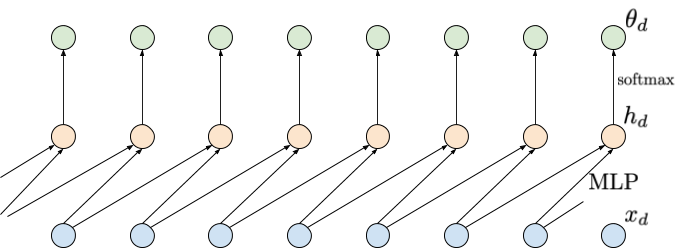
\includegraphics[width=0.5\linewidth]{figs/sequential_MLP}
		 \end{figure}
	\end{block}
	\vspace{-0.4cm}

	\begin{block}{Autoregressive Transformer}
		\begin{minipage}[t]{0.5\columnwidth}
			\begin{figure}
				\centering
	      		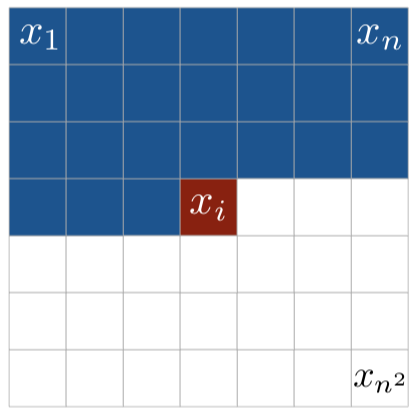
\includegraphics[width=0.6\linewidth]{figs/pixelcnn1}
			\end{figure}
		\end{minipage}%
		\begin{minipage}[t]{0.5\columnwidth}
			\vspace{-0.8cm}
			\begin{figure}
				\centering
		  		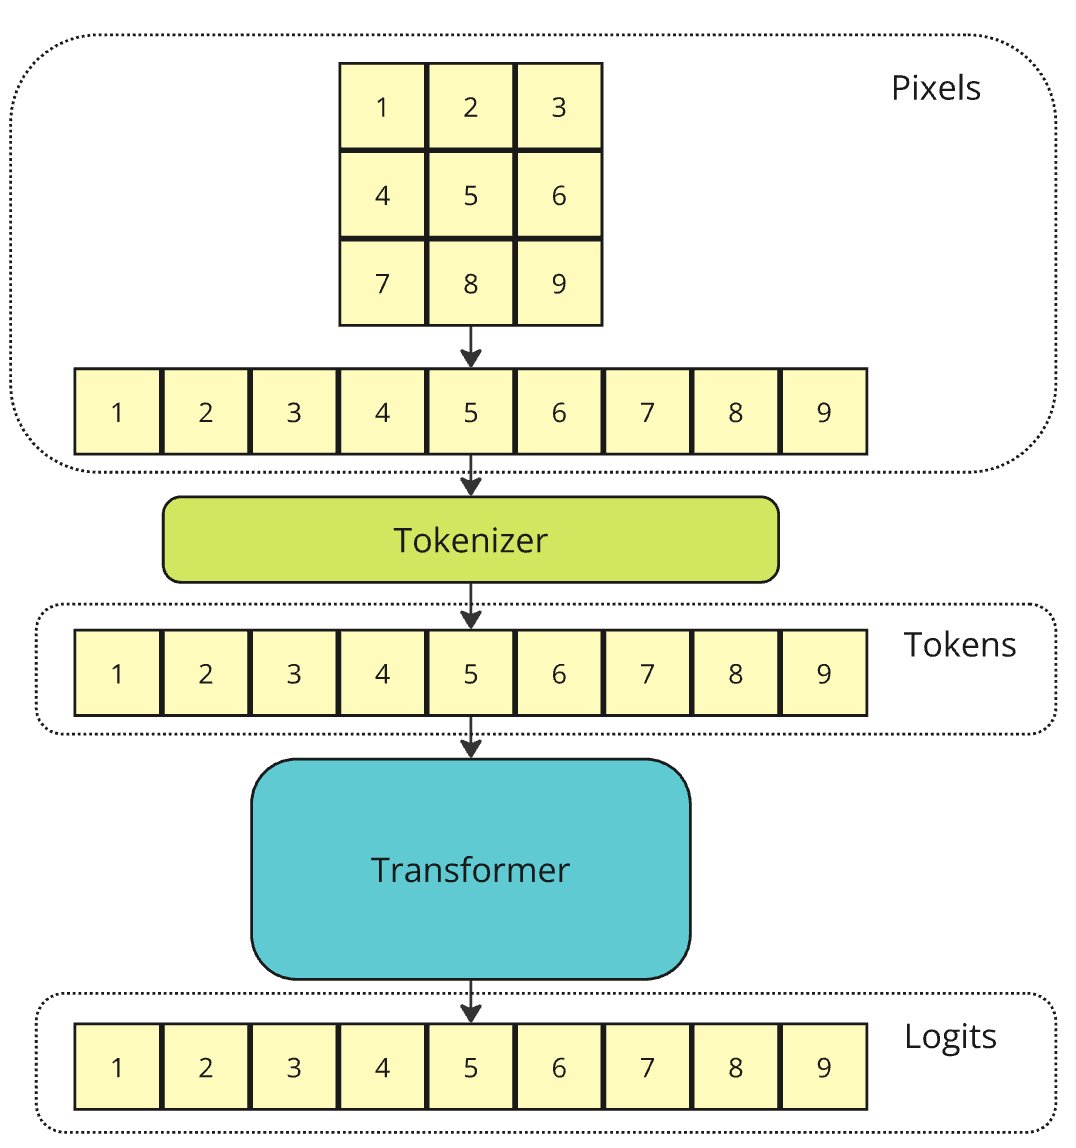
\includegraphics[width=0.8\linewidth]{figs/imagegpt.png}
			\end{figure}
		\end{minipage}
	\end{block}
\end{frame}
%=======
\begin{frame}{Outline}
	\tableofcontents
\end{frame}
%=======
\section{Normalizing Flows (NF)}
%=======
\begin{frame}{Generative Models Zoo}
	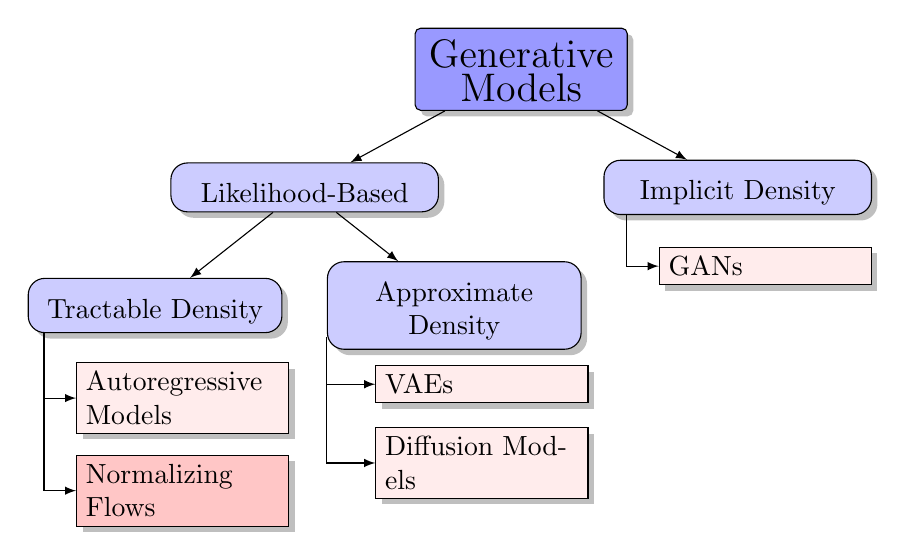
\begin{tikzpicture}[
	 	basic/.style  = {draw, text width=2cm, drop shadow, rectangle},
	 	root/.style   = {basic, rounded corners=2pt, thin, text height=1.1em, text width=7em, align=center, fill=blue!40},
	 	level 1/.style={sibling distance=55mm},
	 	level 2/.style = {basic, rounded corners=6pt, thin, align=center, fill=blue!20, text height=1.1em, text width=9em, sibling distance=38mm},
	 	level 3/.style = {basic, rounded corners=6pt, thin,align=center, fill=blue!20, text width=8.5em},
	 	level 4/.style = {basic, thin, align=left, fill=pink!30, text width=7em},
	 	level 5/.style = {basic, thin, align=left, fill=pink!90, text width=7em},
		edge from parent/.style={->,draw},
		>=latex]
		
		% root of the initial tree, level 1
		\node[root] {\Large Generative Models}
		% The first level, as children of the initial tree
		child {node[level 2] (c1) {Likelihood-Based}
			child {node[level 3] (c11) {Tractable Density}}
			child {node[level 3] (c12) {Approximate Density}}
		}
		child {node[level 2] (c2) {Implicit Density}};
		
		% The second level, relatively positioned nodes
		\begin{scope}[every node/.style={level 4}]
		\node [below of = c11, yshift=-5pt, xshift=10pt] (c111) {Autoregressive Models};
		
		\node [below of = c12, xshift=10pt] (c121) {VAEs};
		\node [below of = c121] (c122) {Diffusion Models};
		\node [below of = c2, xshift=10pt] (c21) {GANs};
		
		\end{scope}
		
		% The second level, relatively positioned nodes
		\begin{scope}[every node/.style={level 5}]
			\node [below of = c111, yshift=-5pt] (c112) {Normalizing Flows};
		\end{scope}
		
		
		% lines from each level 1 node to every one of its "children"
		\foreach \value in {1,2}
		\draw[->] (c11.194) |- (c11\value.west);
		
		\foreach \value in {1,2}
		\draw[->] (c12.194) |- (c12\value.west);
		
		\draw[->] (c2.194) |- (c21.west);
		
	\end{tikzpicture}
\end{frame}
%=======
\begin{frame}{Normalizing Flows: Prerequisites}
	\begin{block}{Jacobian Matrix}
		Let $\bff: \bbR^m \rightarrow \bbR^m$ be a differentiable function.
		\[
			\bz = \bff(\bx), \quad 
			\bJ =  \frac{\partial \bz}{\partial \bx} =
			\begin{pmatrix}
				\frac{\partial z_1}{\partial x_1} & \dots & \frac{\partial z_1}{\partial x_m} \\
				\vdots & \ddots & \vdots \\ 
				\frac{\partial z_m}{\partial x_1} & \dots & \frac{\partial z_m}{\partial x_m}
			\end{pmatrix} \in \bbR^{m \times m}
		\]
		\vspace{-0.3cm}
	\end{block}
    \eqpause
	\begin{block}{Change of Variables Theorem (CoV)}
		Let $\bx$ be a random variable with density $p(\bx)$ and $\bff: \bbR^m \rightarrow \bbR^m$ a differentiable, \textbf{invertible} mapping. If $\bz = \bff(\bx)$ and $\bx = \bff^{-1}(\bz) = \bg(\bz)$, then
		\begin{align*}
			p(\bx) &= p(\bz) |\det(\bJ_{\bff})| = p(\bz) \left|\det \left( \frac{\partial \bz}{\partial \bx} \right) \right| \nextonslide{= p(\bff(\bx)) \left|\det \left(  \frac{\partial \bff(\bx)}{\partial \bx} \right) \right|} \\
			\nextonslide{p(\bz) &= p(\bx) |\det(\bJ_{\bg})| = p(\bx) \left|\det \left(  \frac{\partial \bx}{\partial \bz} \right) \right| = p(\bg(\bz)) \left|\det \left(  \frac{\partial \bg(\bz)}{\partial \bz} \right) \right| }
		\end{align*}
		\vspace{-0.5cm}
	\end{block}
\end{frame}
%=======
\begin{frame}{Jacobian Determinant}
	\myfootnotewithlink{https://jmtomczak.github.io/blog/3/3\_flows.html}{https://jmtomczak.github.io/blog/3/3\_flows.html}
	\begin{block}{Inverse Function Theorem}
		If the function $\bff$ is invertible and its Jacobian is continuous and non-singular, then
		\vspace{-0.3cm}
		\[
		\bJ_{\bff^{-1}} = \bJ_{\bg} = \bJ_\bff^{-1}; \quad \nextonslide{|\det (\bJ_{\bff^{-1}})| = |\det (\bJ_\bg)| = \frac{1}{|\det (\bJ_\bff)|}}
		\]
		\vspace{-0.3cm}
	\end{block}
    \eqpause
	\begin{minipage}{0.55\columnwidth}
		\begin{itemize}
			\item $\bx$ and $\bz$ reside in the same space ($\bbR^m$).
			\vfill
			\item $\bff_{\btheta}(\bx)$ is a parameterized transformation.
			\vfill
			\eqpause
			\item The determinant of the Jacobian $\bJ =\frac{\partial \bff_{\btheta}(\bx)}{\partial \bx}$ quantifies how the volume is changed by the transformation.
		\end{itemize}
	\end{minipage}%
	\begin{minipage}{0.45\columnwidth}
		\begin{figure}
			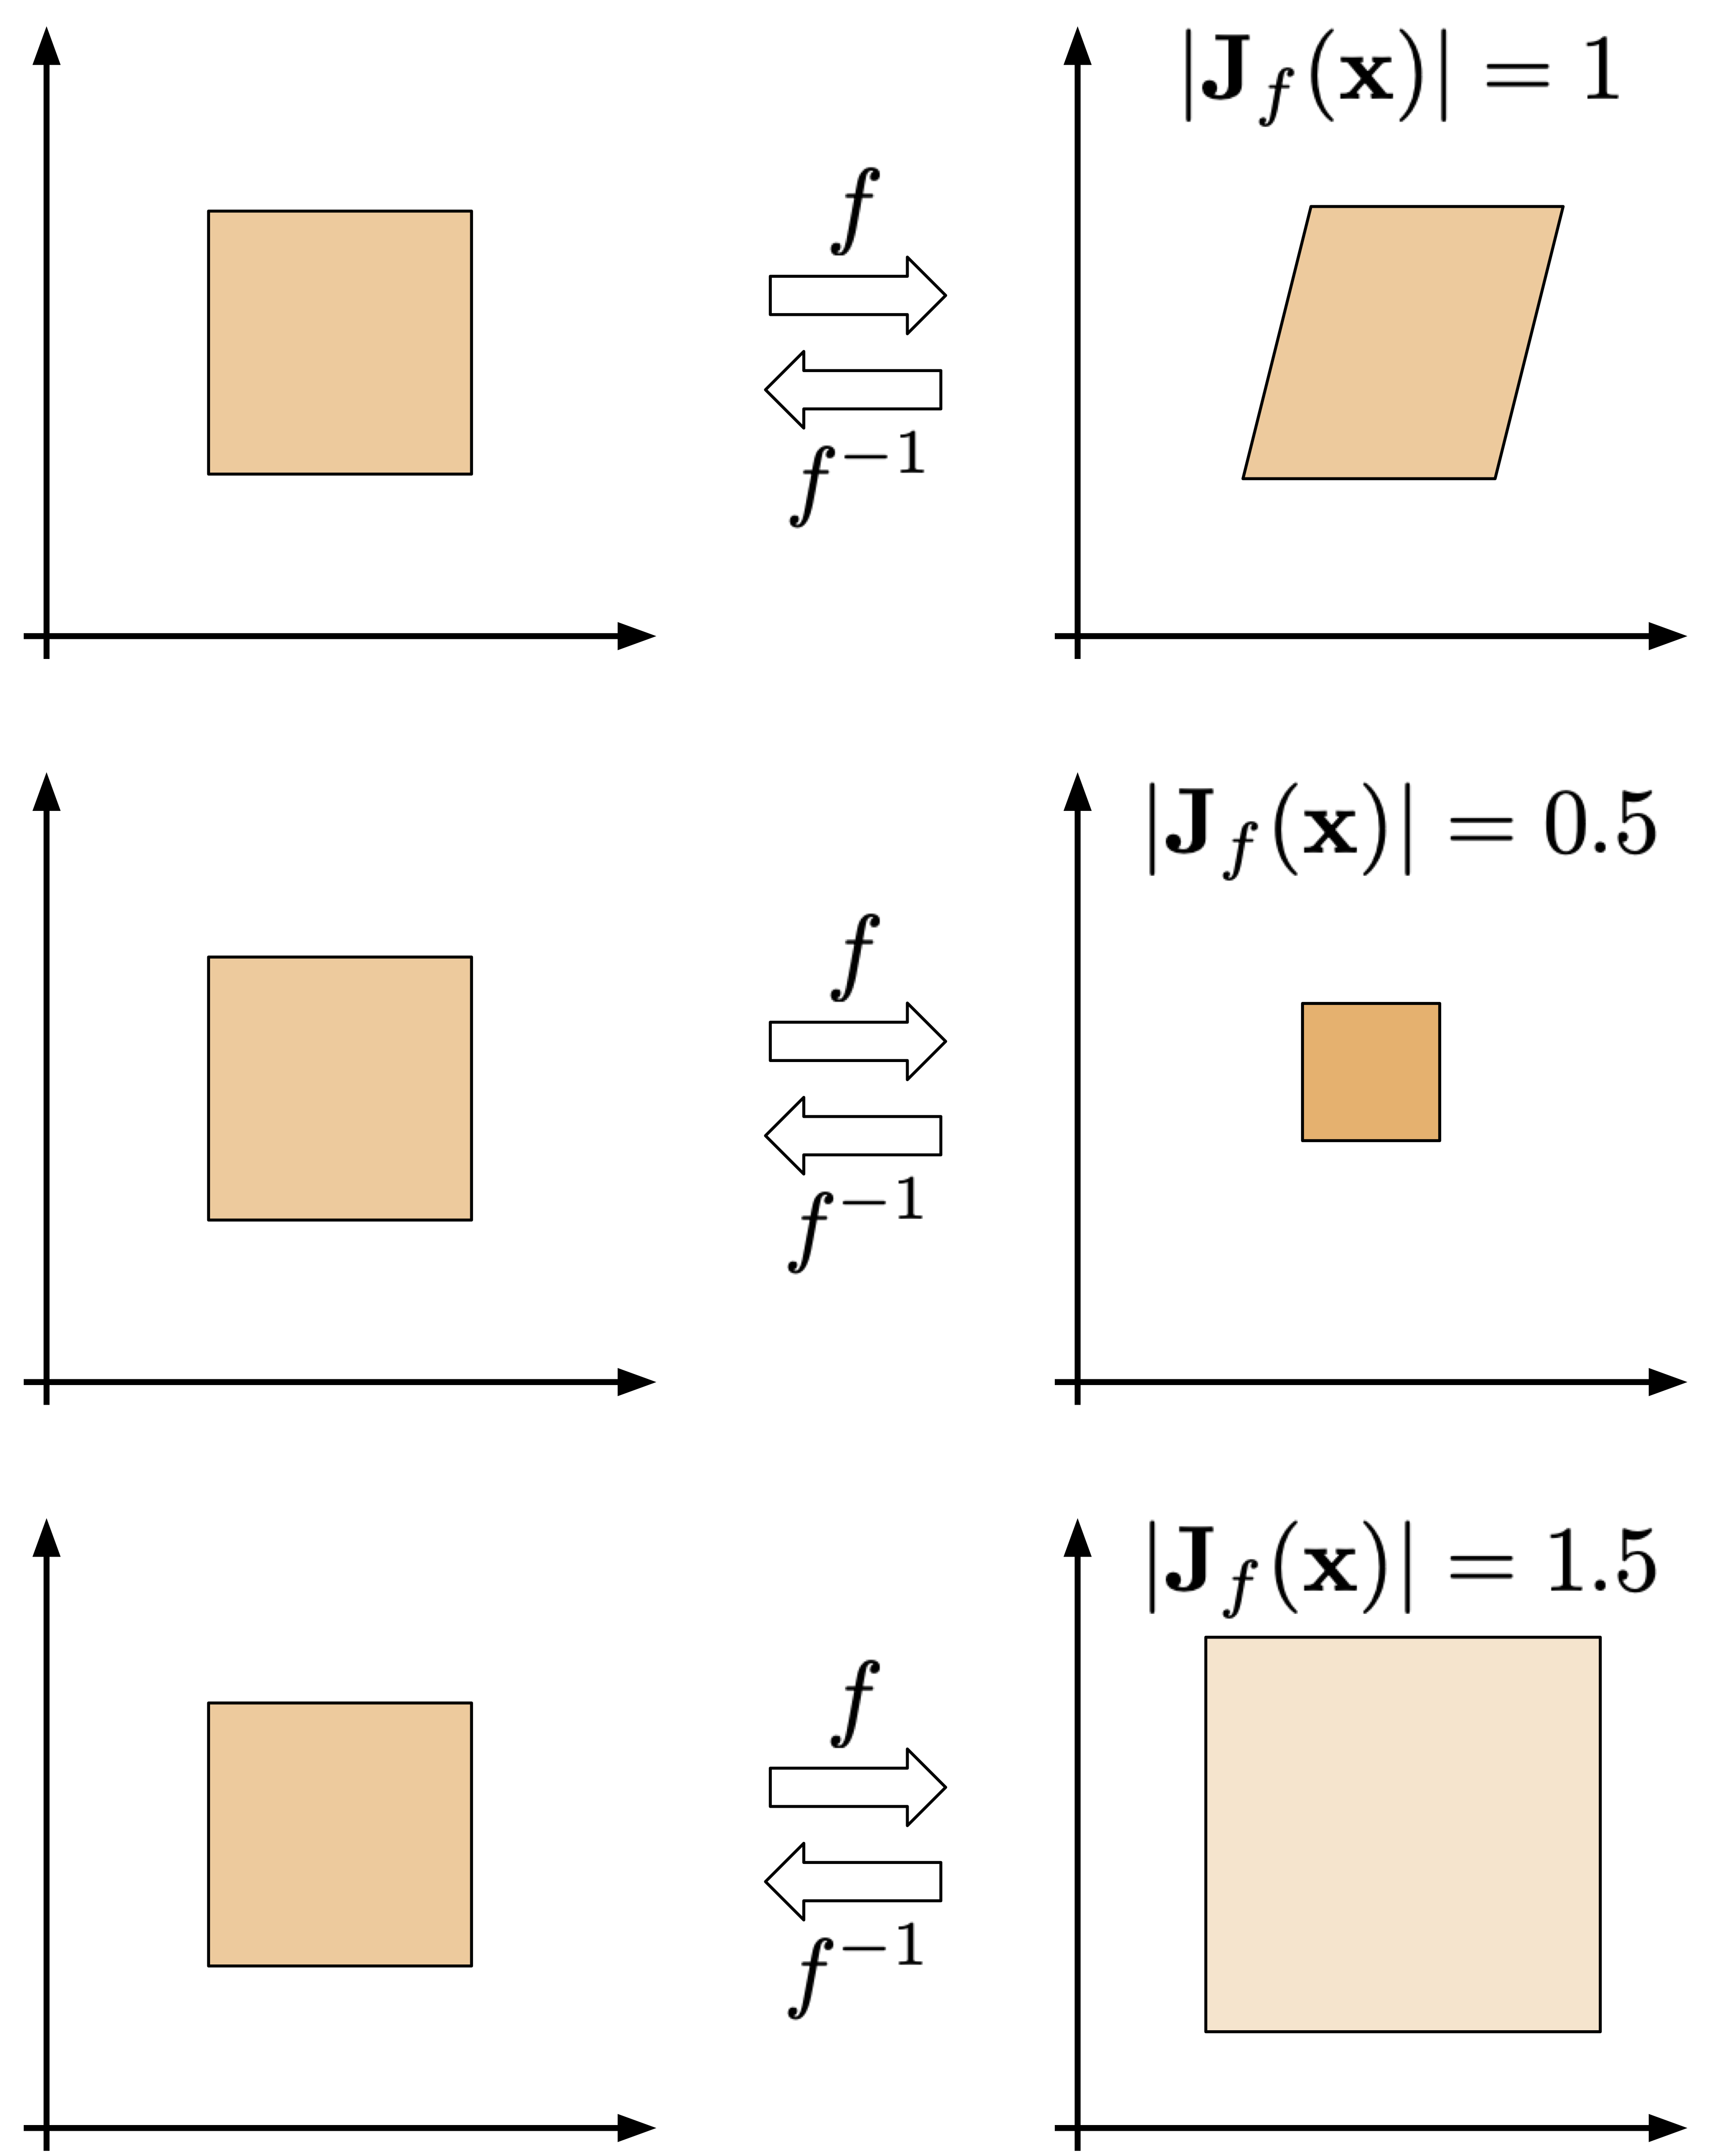
\includegraphics[width=0.8\linewidth]{figs/jacobian_det}
		\end{figure}
	\end{minipage}
\end{frame}
%=======
\begin{frame}{Fitting Normalizing Flows}
	\myfootnotewithlink{https://arxiv.org/abs/1605.08803}{Dinh L., Sohl-Dickstein J., Bengio S. Density Estimation Using Real NVP, 2016} 
	\begin{block}{MLE Problem}
		\vspace{-0.5cm}
		\begin{align*}
			\pt(\bx) &= p(\bz) \left|\det \left(  \frac{\partial \bz}{\partial \bx} \right) \right|  = p(\bff_{\btheta}(\bx)) \left|\det \left( \frac{\partial \bff_{\btheta}(\bx)}{\partial \bx} \right) \right| \\ 
			\nextonslide{\log \pt(\bx) &= \log p(\bff_{\btheta}(\bx)) + \log  |\det (\bJ_{\bff}) | \rightarrow \max_{\btheta}
			}
		\end{align*}
	\end{block}
    \eqpause
	\vspace{-0.2cm}
	\begin{figure}
		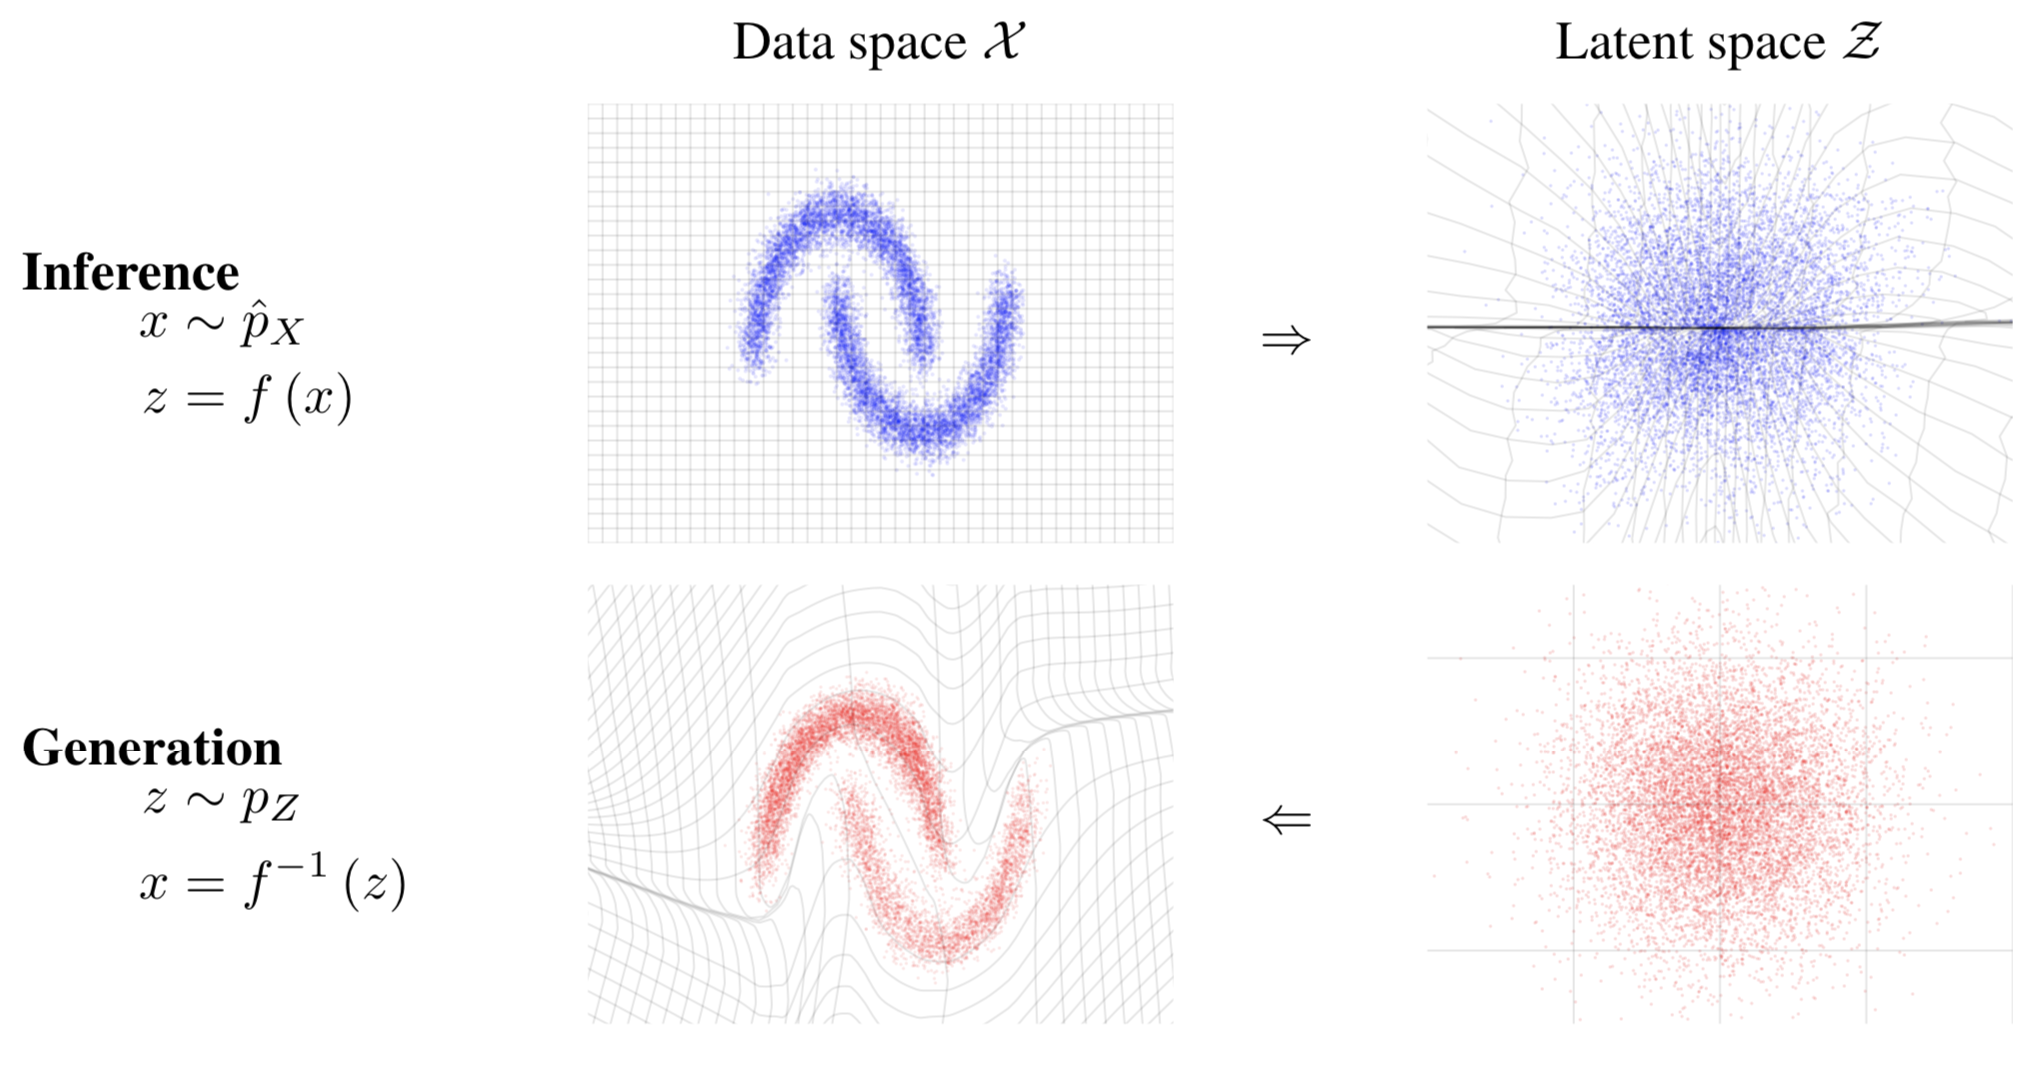
\includegraphics[width=0.85\linewidth]{figs/flows_how2}
	\end{figure}
\end{frame}
%=======
\begin{frame}{Composition of Normalizing Flows}
	\myfootnotewithlink{https://lilianweng.github.io/lil-log/2018/10/13/flow-based-deep-generative-models.html}{https://lilianweng.github.io/lil-log/2018/10/13/flow-based-deep-generative-models.html}
	\vspace{-0.3cm}
	\begin{figure}
		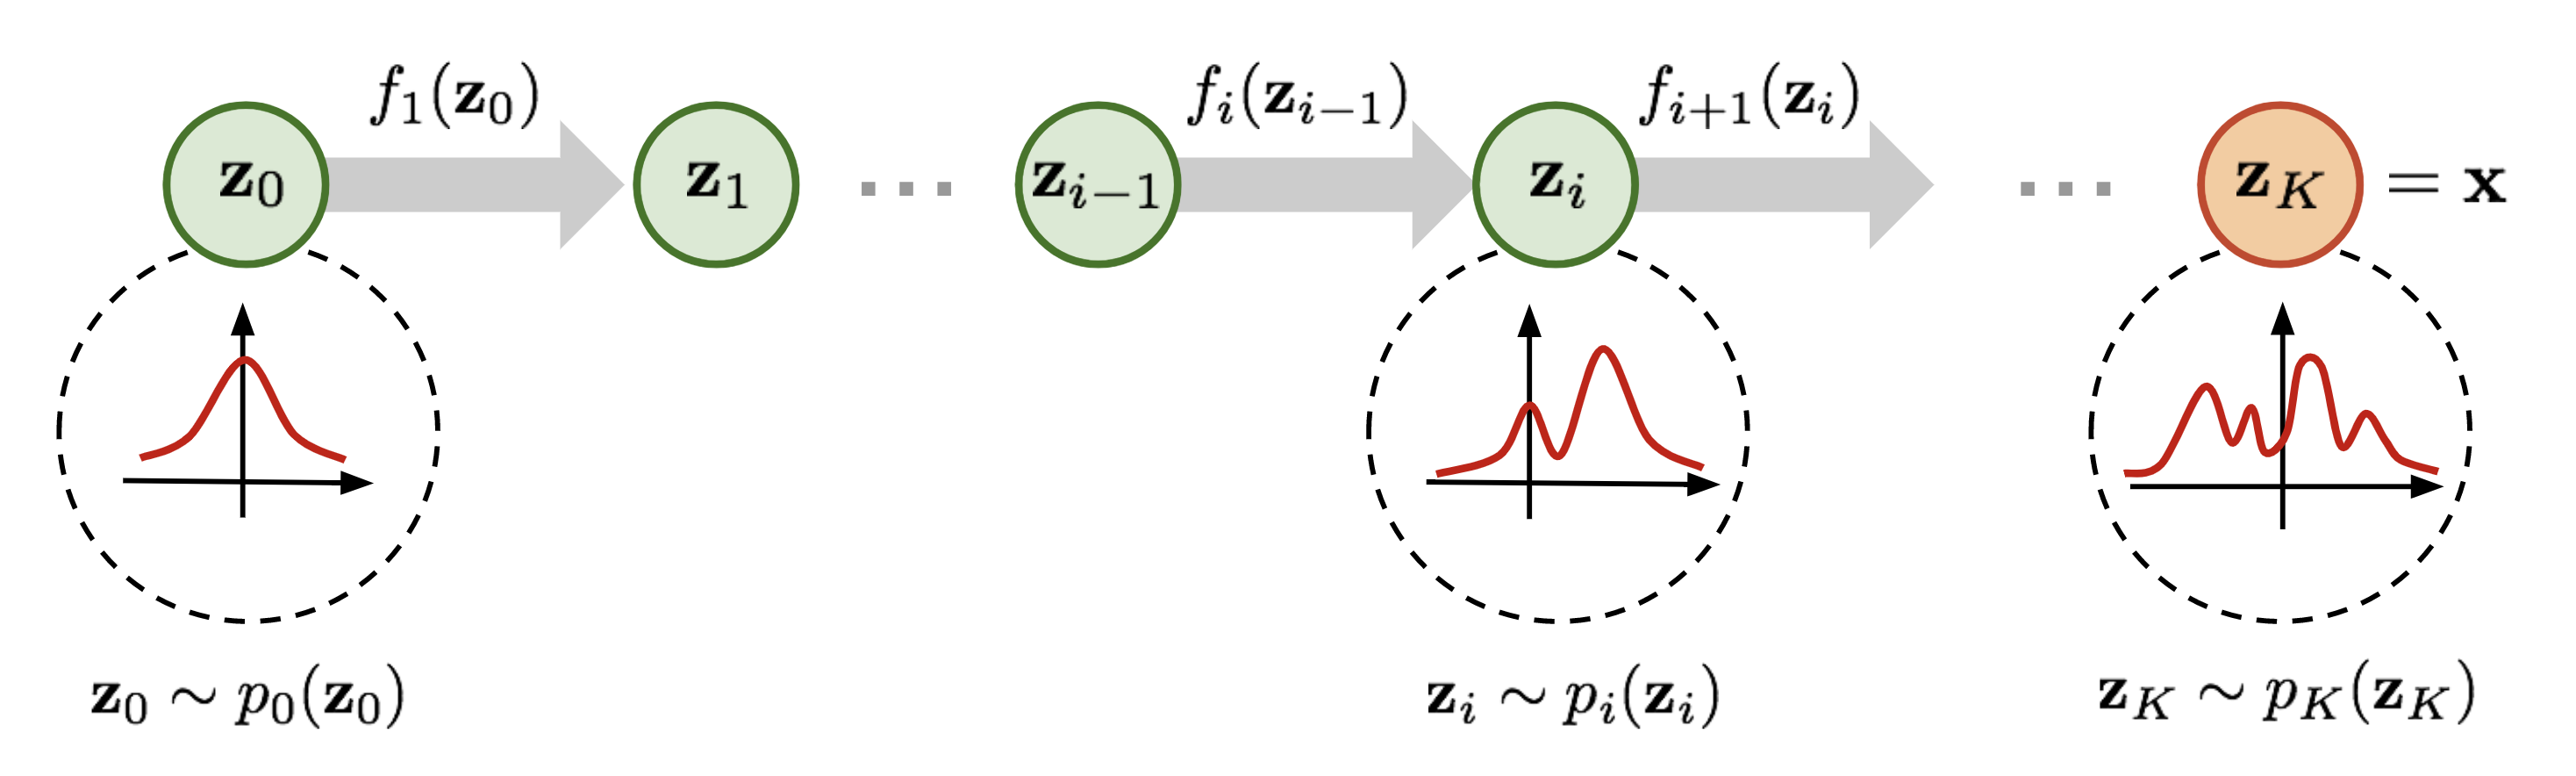
\includegraphics[width=0.95\linewidth]{figs/normalizing-flow}
	\end{figure}
	\vspace{-0.3cm}
	\eqpause
	\begin{block}{Theorem}
		If every $\{\bff_k\}_{k=1}^K$ satisfies the conditions of the change-of-variables theorem, then the composition $\bff(\bx) = \bff_K \circ \ldots \circ \bff_1(\bx)$ also satisfies them.
	\end{block}
	\vspace{-0.3cm}
	{\footnotesize
		\begin{multline*}
			\pt(\bx) = p(\bff(\bx)) \left|\det \left(\frac{\partial \bff(\bx)}{\partial \bx} \right) \right| 
			\nextonslide{=p(\bff(\bx)) \left|\det \left(\frac{\partial \bff_K}{\partial \bff_{K-1}} \dots \frac{\partial \bff_1}{\partial \bx} \right) \right|}
			\nextonslide{= \\ = p(\bff(\bx)) \prod_{k=1}^K \left|\det \left(\frac{\partial \bff_{k}}{\partial \bff_{k-1}} \right) \right|
			= p(\bff(\bx)) \prod_{k=1}^K |\det ( \bJ_{\bff_k}) |}
		\end{multline*}
	}
\end{frame}
%=======
\begin{frame}{Normalizing Flows (NF)}
	\vspace{-0.3cm}
	\[
		\log \pt(\bx) = \log p(\bff_{\btheta}(\bx)) + \log |\det (\bJ_\bff)|
	\]
	\vspace{-0.4cm}
	\begin{block}{Definition}
		A normalizing flow is a \textit{differentiable, invertible} mapping that transforms data $\bx$ to latent noise $\bz$.
	\end{block}
    \eqpause
	\begin{itemize}
		\item \textbf{Normalizing} refers to mapping samples from $\pd(\bx)$ to a base distribution $p(\bz)$.
		\item \textbf{Flow} describes the sequence of transformations that maps samples from $p(\bz)$ to the target, more complex distribution.
		\[
			\bz = \bff_K \circ \ldots \circ \bff_1(\bx); \quad \bx = \bff_1^{-1} \circ \ldots \circ \bff_K^{-1} (\bz) = \bg_1 \circ \ldots \circ \bg_K(\bz)
		\] 
		\vspace{-0.4cm}
		\eqpause
		\begin{block}{Log-Likelihood}
			\vspace{-0.5cm}
			\[
				\log \pt(\bx) = \log p(\bff_K \circ \ldots \circ \bff_1(\bx)) + \sum_{k=1}^K \log |\det (\bJ_{\bff_k})|
			\]
			\vspace{-0.4cm} \\
			where $\bJ_{\bff_k} = \frac{\partial \bff_k}{\partial \bff_{k-1}}$.
		\end{block}
	\end{itemize}
	\eqpause
	\textbf{Note:} Here we consider only \textbf{continuous} random variables.
\end{frame}
%=======
\begin{frame}{Normalizing Flows}
	\myfootnotewithlink{https://arxiv.org/abs/1912.02762}{Papamakarios G. et al. Normalizing Flows for Probabilistic Modeling and Inference, 2019} 
	\begin{block}{Example: 4-Step NF}
		\vspace{-0.2cm}
		\begin{figure}
			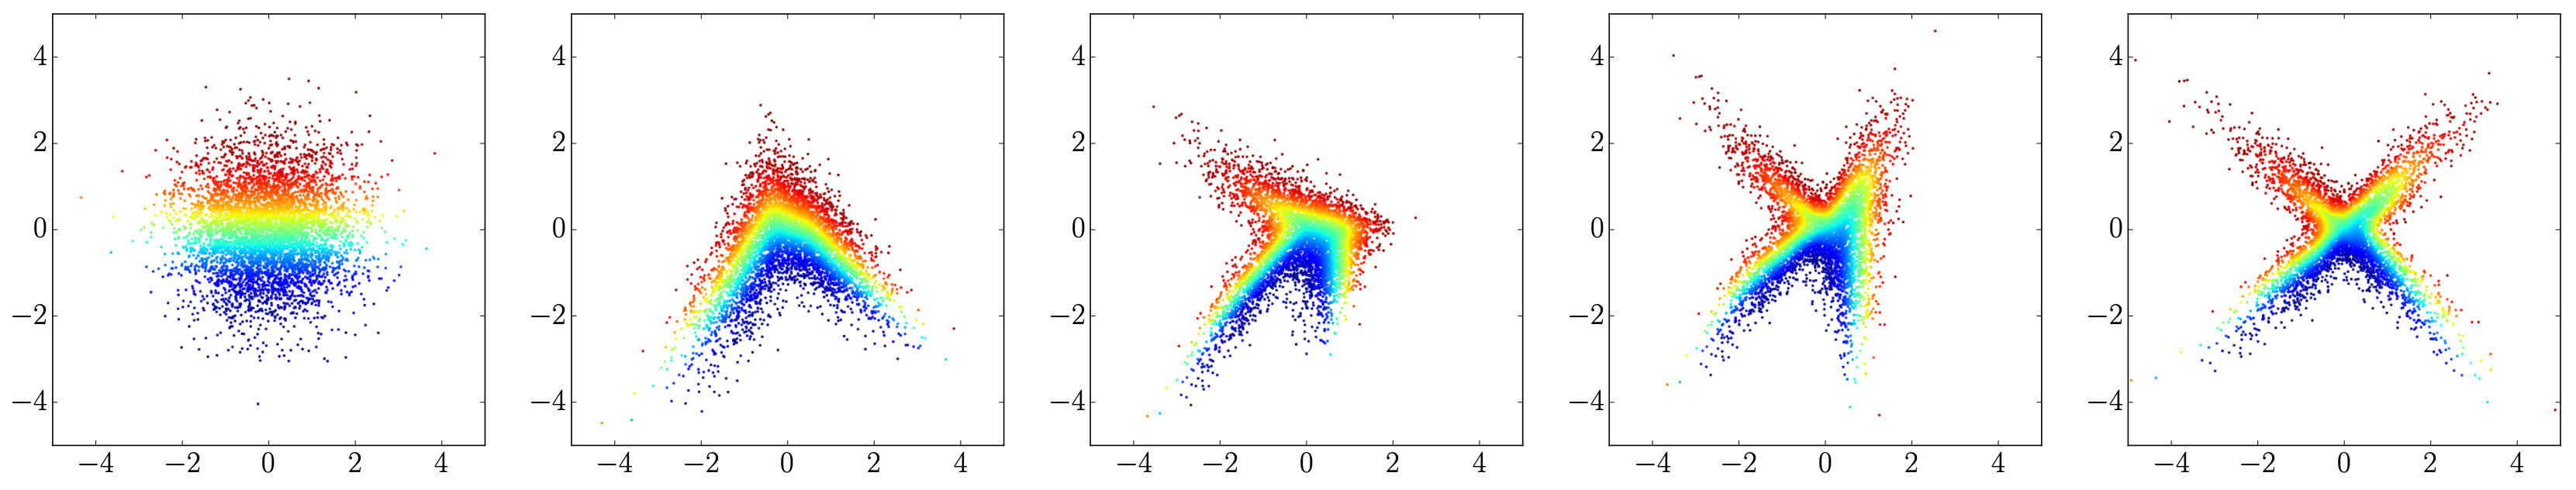
\includegraphics[width=\linewidth]{figs/flow_4_steps_example.png}
		\end{figure}
	\end{block}
    \eqpause
	\vspace{-0.5cm}
	\begin{block}{NF Log-Likelihood}
		\vspace{-0.3cm}
		\[
			\log \pt(\bx) = \log p(\bff_{\btheta}(\bx)) + \log |\det ( \bJ_\bff)|
		\]
		\vspace{-0.5cm}
	\end{block}
	What's the computational complexity of evaluating this determinant?
    \eqpause
	\begin{block}{Requirements}
		\begin{itemize}
			\item Efficient computation of the Jacobian $\bJ_\bff = \frac{\partial \bff_{\btheta}(\bx)}{\partial \bx}$
			\item Efficient inversion of the transformation $\bff_{\btheta}(\bx)$
		\end{itemize}
	\end{block}
\end{frame}
%=======
\section{NF Examples}
%=======
\subsection{Linear Normalizing Flows}
%=======
\begin{frame}{Jacobian Structure}
	\begin{block}{Normalizing Flows Log-Likelihood}
		\[
			\log \pt(\bx) = \log p(\bff_{\btheta}(\bx)) + \log \left|\det \left( \frac{\partial \bff_{\btheta}(\bx)}{\partial \bx} \right) \right|
		\]
	\end{block}
	The principal computational challenge is evaluating the Jacobian determinant.
    \eqpause
	\begin{block}{What is $\det(\bJ)$ in These Cases?}
		Consider a linear layer $\bz = \bW \bx$, $\bW \in \bbR^{m \times m}$.
		\begin{enumerate}
			\item $\bz$ is a permutation of $\bx$.
			    \eqpause
			\item $z_j$ depends only on $x_j$. 
			\vspace{-0.3cm}
			\[
				\nextonslide{\log \left|\det \left( \frac{\partial \bff_{\btheta}(\bx)}{\partial \bx} \right) \right| = \log \left| \prod_{j=1}^m \frac{\partial f_{j, \btheta}(x_j)}{\partial x_j} \right| = \sum_{j=1}^m \log \left|  \frac{\partial f_{j, \btheta}(x_j)}{\partial x_j} \right|}
			\]
			\eqpause
			\item $z_j$ depends only on $\bx_{1:j}$ (autoregressive dependency).
		\end{enumerate}
	\end{block}
\end{frame}
%=======
\begin{frame}{Linear Normalizing Flows}
	\myfootnotewithlink{https://arxiv.org/abs/1807.03039}{Kingma D. P., Dhariwal P. Glow: Generative Flow with Invertible 1x1 Convolutions, 2018} 
	\[
		\bz = \bff_{\btheta}(\bx) = \bW \bx, \quad \bW \in \bbR^{m \times m}, \quad \btheta = \bW, \quad \bJ_\bff = \bW^T
	\]
	In general, matrix inversion has computational complexity $O(m^3)$.
    \eqpause
	\begin{block}{Invertibility}
		\begin{itemize}
			\item Diagonal matrix: $O(m)$.
			\item Triangular matrix: $O(m^2)$.
			\item Directly parameterizing the full group of invertible matrices is infeasible.
		\end{itemize}
	\end{block}
    \eqpause
	\begin{block}{Invertible $1 \times 1$ Convolution}
		$\bW \in \bbR^{c \times c}$ acts as the kernel of a $1 \times 1$ convolution with $c$ input and $c$ output channels. 
		Calculating or differentiating $\det (\bW)$ incurs a cost of $O(c^3)$.
		It is critical that $\bW$ is invertible.
	\end{block}
	
\end{frame}
%=======
\begin{frame}{Linear Normalizing Flows}
	\myfootnote{\href{https://arxiv.org/abs/1807.03039}{Kingma D. P., et al. Glow: Generative Flow with Invertible 1x1 Convolutions, 2018}  \\
	\href{https://arxiv.org/abs/1901.11137}{Hoogeboom E., et al. Emerging Convolutions for Generative Normalizing Flows, 2019}
	}
	\vspace{-0.3cm}
	\[
		\bz = \bff_{\btheta}(\bx) = \bW \bx, \quad \bW \in \bbR^{m \times m}, \quad \btheta = \bW, \quad \bJ_\bff = \bW^T
	\]
	\vspace{-0.7cm}
	\eqpause
	\begin{block}{Matrix Decompositions}
		\begin{itemize}
			\item \textbf{LU Decomposition:}
			\vspace{-0.3cm}
			\[
				\bW = \bP \bL \bU,
			\]
			\vspace{-0.7cm} \\
			where $\bP$ is a permutation matrix, $\bL$ is lower triangular with positive diagonal, and $\bU$ is upper triangular with positive diagonal.
			\eqpause
			\item \textbf{QR Decomposition:}
			\vspace{-0.3cm}
			\[
				\bW = \bQ \bR,
			\]
			\vspace{-0.7cm} \\
			where $\bQ$ is orthogonal, and $\bR$ is upper triangular with positive diagonal.
		\end{itemize}
	\end{block}
    \eqpause
	Decomposition is performed only at initialization; the decomposed matrices ($\bP, \bL, \bU$ or $\bQ, \bR$) are optimized during training.

\end{frame}
%=======
\subsection{Gaussian Autoregressive NF}
%=======
\begin{frame}{Gaussian Autoregressive Model}
	\myfootnotewithlink{https://arxiv.org/abs/1606.04934}{Kingma D. P. et al. Improving Variational Inference with Inverse Autoregressive Flow, 2016} 
	Consider the autoregressive model:
	\vspace{-0.3cm}
	{\small
		\[
		\pt(\bx) = \prod_{j=1}^m \pt(x_j | \bx_{1:j-1}), \quad
		\pt(x_j | \bx_{1:j-1}) = \cN \left(\mu_{j, \btheta}(\bx_{1:j-1}), \sigma^2_{j, \btheta} (\bx_{1:j-1})\right)
		\]
	}
	\vspace{-0.5cm}
	\eqpause
	\begin{block}{Sampling}
		\vspace{-0.3cm}
		\[
		x_j = \sigma_{j, \btheta} (\bx_{1:j-1}) \cdot z_j + \mu_{j, \btheta}(\bx_{1:j-1}), \quad z_j \sim \cN(0, 1)
		\]
		\vspace{-0.7cm}
	\end{block}
	\eqpause
	\begin{block}{Inverse Transformation}
		\vspace{-0.5cm}
		\[
		z_j = \frac{x_j - \mu_{j, \btheta}(\bx_{1:j-1})}{\sigma_{j, \btheta} (\bx_{1:j-1}) }
		\]
		\vspace{-0.4cm}
	\end{block}
	\eqpause
	\begin{itemize}
		\item This gives an \textbf{invertible} and \textbf{differentiable} transformation from $p(\bz)$ to $\pt(\bx)$.
		    \eqpause
		\item This model is called an autoregressive (AR) NF with base distribution $p(\bz) = \cN(0, \bI)$.
		    \eqpause
		\item The Jacobian matrix of this transformation is triangular.
	\end{itemize}
\end{frame}
%=======
\begin{frame}{Gaussian Autoregressive NF}
	\myfootnotewithlink{https://arxiv.org/abs/1705.07057}{Papamakarios G., Pavlakou T., Murray I. Masked Autoregressive Flow for Density Estimation, 2017}
	\vspace{-0.5cm}
	\begin{align*}
		\bx &= \bg_{\btheta}(\bz) \quad \Rightarrow \quad {\color{violet} x_j} = \sigma_{j, \btheta} ({\color{violet} \bx_{1:j-1}}) \cdot {\color{teal} z_j} + \mu_{j, \btheta}({\color{violet} \bx_{1:j-1}}) \\
		\bz &= \bff_{\btheta}(\bx) \quad \Rightarrow \quad {\color{teal} z_j} = \frac{{\color{violet}x_j} - \mu_{j, \btheta}({\color{violet}\bx_{1:j-1}})}{ \sigma_{j, \btheta} ({\color{violet}\bx_{1:j-1}})}
	\end{align*}
	\eqpause
	To generate samples, apply $\bg_{\btheta}(\bz)$ sequentially;\\
	inference via $\bff_{\btheta}(\bx)$ is parallelizable.
	\eqpause

	\begin{block}{Forward KL for NFs}
		\vspace{-0.2cm}
		\[
			\KL(\pd \| \pt)  = -\bbE_{\pd(\bx)} \left[\log p(\bff_{\btheta}(\bx)) + \log  |\det (\bJ_\bff)|\right] + \text{const}
		\]
		\vspace{-0.5cm}
		\eqpause
		\begin{itemize}
			\item Computing $\bff_{\btheta}(\bx)$ and its Jacobian is necessary.
			\item One must be able to evaluate the density $p(\bz)$.
			\item The inverse $\bg_{\btheta}(\bz) = \bff_{\btheta}^{-1}(\bz)$ is only needed for sampling.
		\end{itemize}
	\end{block}
\end{frame}
%=======
\begin{frame}{Gaussian Autoregressive NF}
	\myfootnotewithlink{https://blog.evjang.com/2018/01/nf2.html}{Image credit: https://blog.evjang.com/2018/01/nf2.html}
	\vspace{-0.5cm}
	\begin{align*}
		\bx &= \bg_{\btheta}(\bz) \quad \Rightarrow \quad {\color{violet} x_j} = \sigma_{j, \btheta} ({\color{violet} \bx_{1:j-1}}) \cdot {\color{teal} z_j} + \mu_{j, \btheta}({\color{violet} \bx_{1:j-1}}) \\
		\bz &= \bff_{\btheta}(\bx) \quad \Rightarrow \quad {\color{teal} z_j} = \frac{{\color{violet}x_j} - \mu_{j, \btheta}({\color{violet}\bx_{1:j-1}})}{\sigma_{j, \btheta} ({\color{violet}\bx_{1:j-1}})}
	\end{align*}
	\vspace{-0.5cm}
	\eqpause
	\begin{itemize}
		\item Sampling must be done sequentially, but density estimation can be parallelized.
		\item The forward KL divergence is a natural objective for training.
	\end{itemize}
	\vspace{-0.3cm}
	\eqpause
	\begin{minipage}[t]{0.65\columnwidth}
		\begin{block}{Forward Transformation: $\bff_{\btheta}(\bx)$}
			\[
				z_j = \frac{x_j - \mu_{j, \btheta}(\bx_{1:j-1})}{\sigma_{j, \btheta} (\bx_{1:j-1}) }
			\]
			\vspace{-0.4cm}
		\end{block}
	\end{minipage}% 
	\begin{minipage}[t]{0.35\columnwidth}
		\begin{figure}[h]
			\centering
			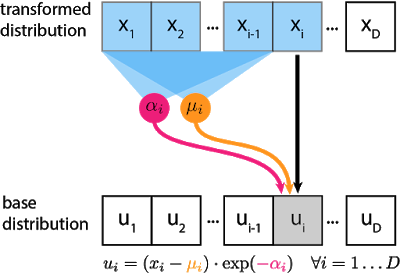
\includegraphics[width=.9\linewidth]{figs/af_iaf_explained_2.png}
		\end{figure}
	\end{minipage} \\
	\eqpause
	\begin{minipage}[t]{0.65\columnwidth}
		\begin{block}{Inverse Transformation: $\bg_{\btheta}(\bz)$}
			\vspace{-0.5cm}
			\[
				x_j = \sigma_{j, \btheta} (\bx_{1:j-1}) \cdot z_j + \mu_{j, \btheta}(\bx_{1:j-1})
			\]
		\end{block}
	\end{minipage}%
	\begin{minipage}[t]{0.35\columnwidth}
		\begin{figure}[h]
			\centering
			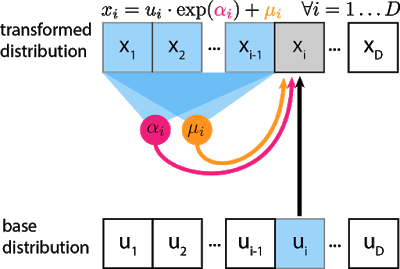
\includegraphics[width=.9\linewidth]{figs/af_iaf_explained_1.png}
		\end{figure}
	\end{minipage}
\end{frame}
%=======
\subsection{Coupling Layer (RealNVP)}
%=======
\begin{frame}{RealNVP}
	\myfootnotewithlink{https://arxiv.org/abs/1605.08803}{Dinh L., Sohl-Dickstein J., Bengio S. Density Estimation Using Real NVP, 2016} 
	\vspace{-0.5cm}

	Split $\bx$ and $\bz$ into two parts: 
	\[
		\bx = [\bx_1, \bx_2] = [\bx_{1:d}, \bx_{d+1:m}]; \quad \bz = [\bz_1, \bz_2] = [\bz_{1:d}, \bz_{d+1:m}]
	\]
	\vspace{-0.7cm}
	\eqpause
	\begin{block}{Coupling Layer}
		\vspace{-0.7cm}
		\[
				\begin{cases} \bx_1 = \bz_1 \\ \bx_2 = \bz_2 \odot \bsigma_{\btheta}(\bz_1) + \bmu_{\btheta}(\bz_1) \end{cases}
				\qquad
				\nextonslide{
				\begin{cases} \bz_1 = \bx_1 \\ \bz_2 = (\bx_2 - \bmu_{\btheta}(\bx_1)) \odot \frac{1}{\bsigma_{\btheta}(\bx_1)} \end{cases}
				}
		\]
	\end{block}
	\vspace{-0.5cm}
	\eqpause
	\begin{block}{Image Partitioning}
		
		\begin{minipage}[t]{0.5\columnwidth}
			\begin{figure}
				\centering
				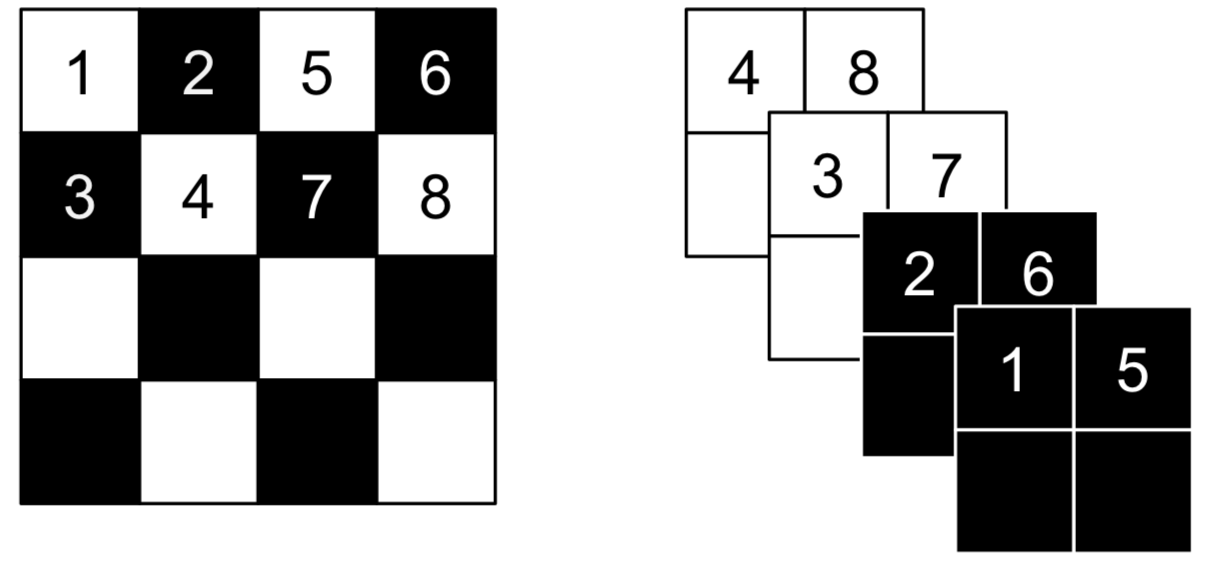
\includegraphics[width=\linewidth]{figs/realnvp_masking.png}
			\end{figure}
		\end{minipage}% 
		\begin{minipage}[t]{0.5\columnwidth}
			\begin{itemize}
				\item Checkerboard ordering corresponds to masking.
				\item Channelwise ordering relies on splitting.
			\end{itemize}
		\end{minipage}
	\end{block}
	\vspace{-0.5cm}
\end{frame}
%=======
\begin{frame}{RealNVP}
	\myfootnotewithlink{https://arxiv.org/abs/1605.08803}{Dinh L., Sohl-Dickstein J., Bengio S. Density Estimation Using Real NVP, 2016} 
	\begin{block}{Coupling Layer}
		\vspace{-0.7cm}
		\[
		 \begin{cases} {\color{violet}\bx_1} = {\color{teal}\bz_1} \\ {\color{violet}\bx_2} = {\color{teal}\bz_2} \odot \bsigma_{\btheta}({\color{teal}\bz_1}) + \bmu_{\btheta}({\color{teal}\bz_1}) \end{cases}
			\qquad
		\begin{cases} {\color{teal}\bz_1} ={\color{violet} \bx_1} \\ {\color{teal}\bz_2} = ({\color{violet}\bx_2} - \bmu_{\btheta}({\color{violet}\bx_1})) \odot \frac{1}{\bsigma_{\btheta}({\color{violet}\bx_1})} \end{cases}
		\]
		In both training and sampling, only a single forward pass is needed!
	\end{block}
	\eqpause
	\vspace{-0.3cm}
	\begin{block}{Jacobian}
		\vspace{-0.5cm}
		\[
			\det \left( \frac{\partial \bz}{\partial \bx} \right) = \det 
			\begin{pmatrix}
				\bI_d & 0_{d \times m-d} \\
				\frac{\partial \bz_2}{\partial \bx_1} & \frac{\partial \bz_2}{\partial \bx_2}
			\end{pmatrix} \nextonslide{ = \prod_{j=1}^{m-d} \frac{1}{\sigma_{j, \btheta}(\bx_1)}}
		\]
		\vspace{-0.5cm}
	\end{block}
	\eqpause
	\begin{block}{Gaussian AR NF}
		\vspace{-0.7cm}
		\begin{align*}
				\bx &= \bg_{\btheta}(\bz) \quad \Rightarrow \quad {\color{violet}x_j} = \sigma_{j, \btheta} ({\color{violet}\bx_{1:j-1}}) \cdot {\color{teal} z_j} + \mu_{j, \btheta}({\color{violet}\bx_{1:j-1}}) \\
				\bz &= \bff_{\btheta}(\bx) \quad \Rightarrow \quad {\color{teal} z_j} = \left({\color{violet} x_j} - \mu_{j, \btheta}({\color{violet}\bx_{1:j-1}}) \right) \cdot \frac{1}{\sigma_{j, \btheta} ({\color{violet} \bx_{1:j-1}}) }.
		\end{align*}
		\vspace{-0.5cm}
	\end{block}
	How can the RealNVP layer be derived as a special instance of the Gaussian autoregressive NF?
	
\end{frame}
%=======
\begin{frame}{Glow: Coupling Layers + Linear Flows ($1 \times 1$ Convolutions)}
	\myfootnotewithlink{https://arxiv.org/abs/1807.03039}{Kingma D. P., Dhariwal P. Glow: Generative Flow with Invertible 1x1 Convolutions, 2018}
	\begin{figure}
		\centering
		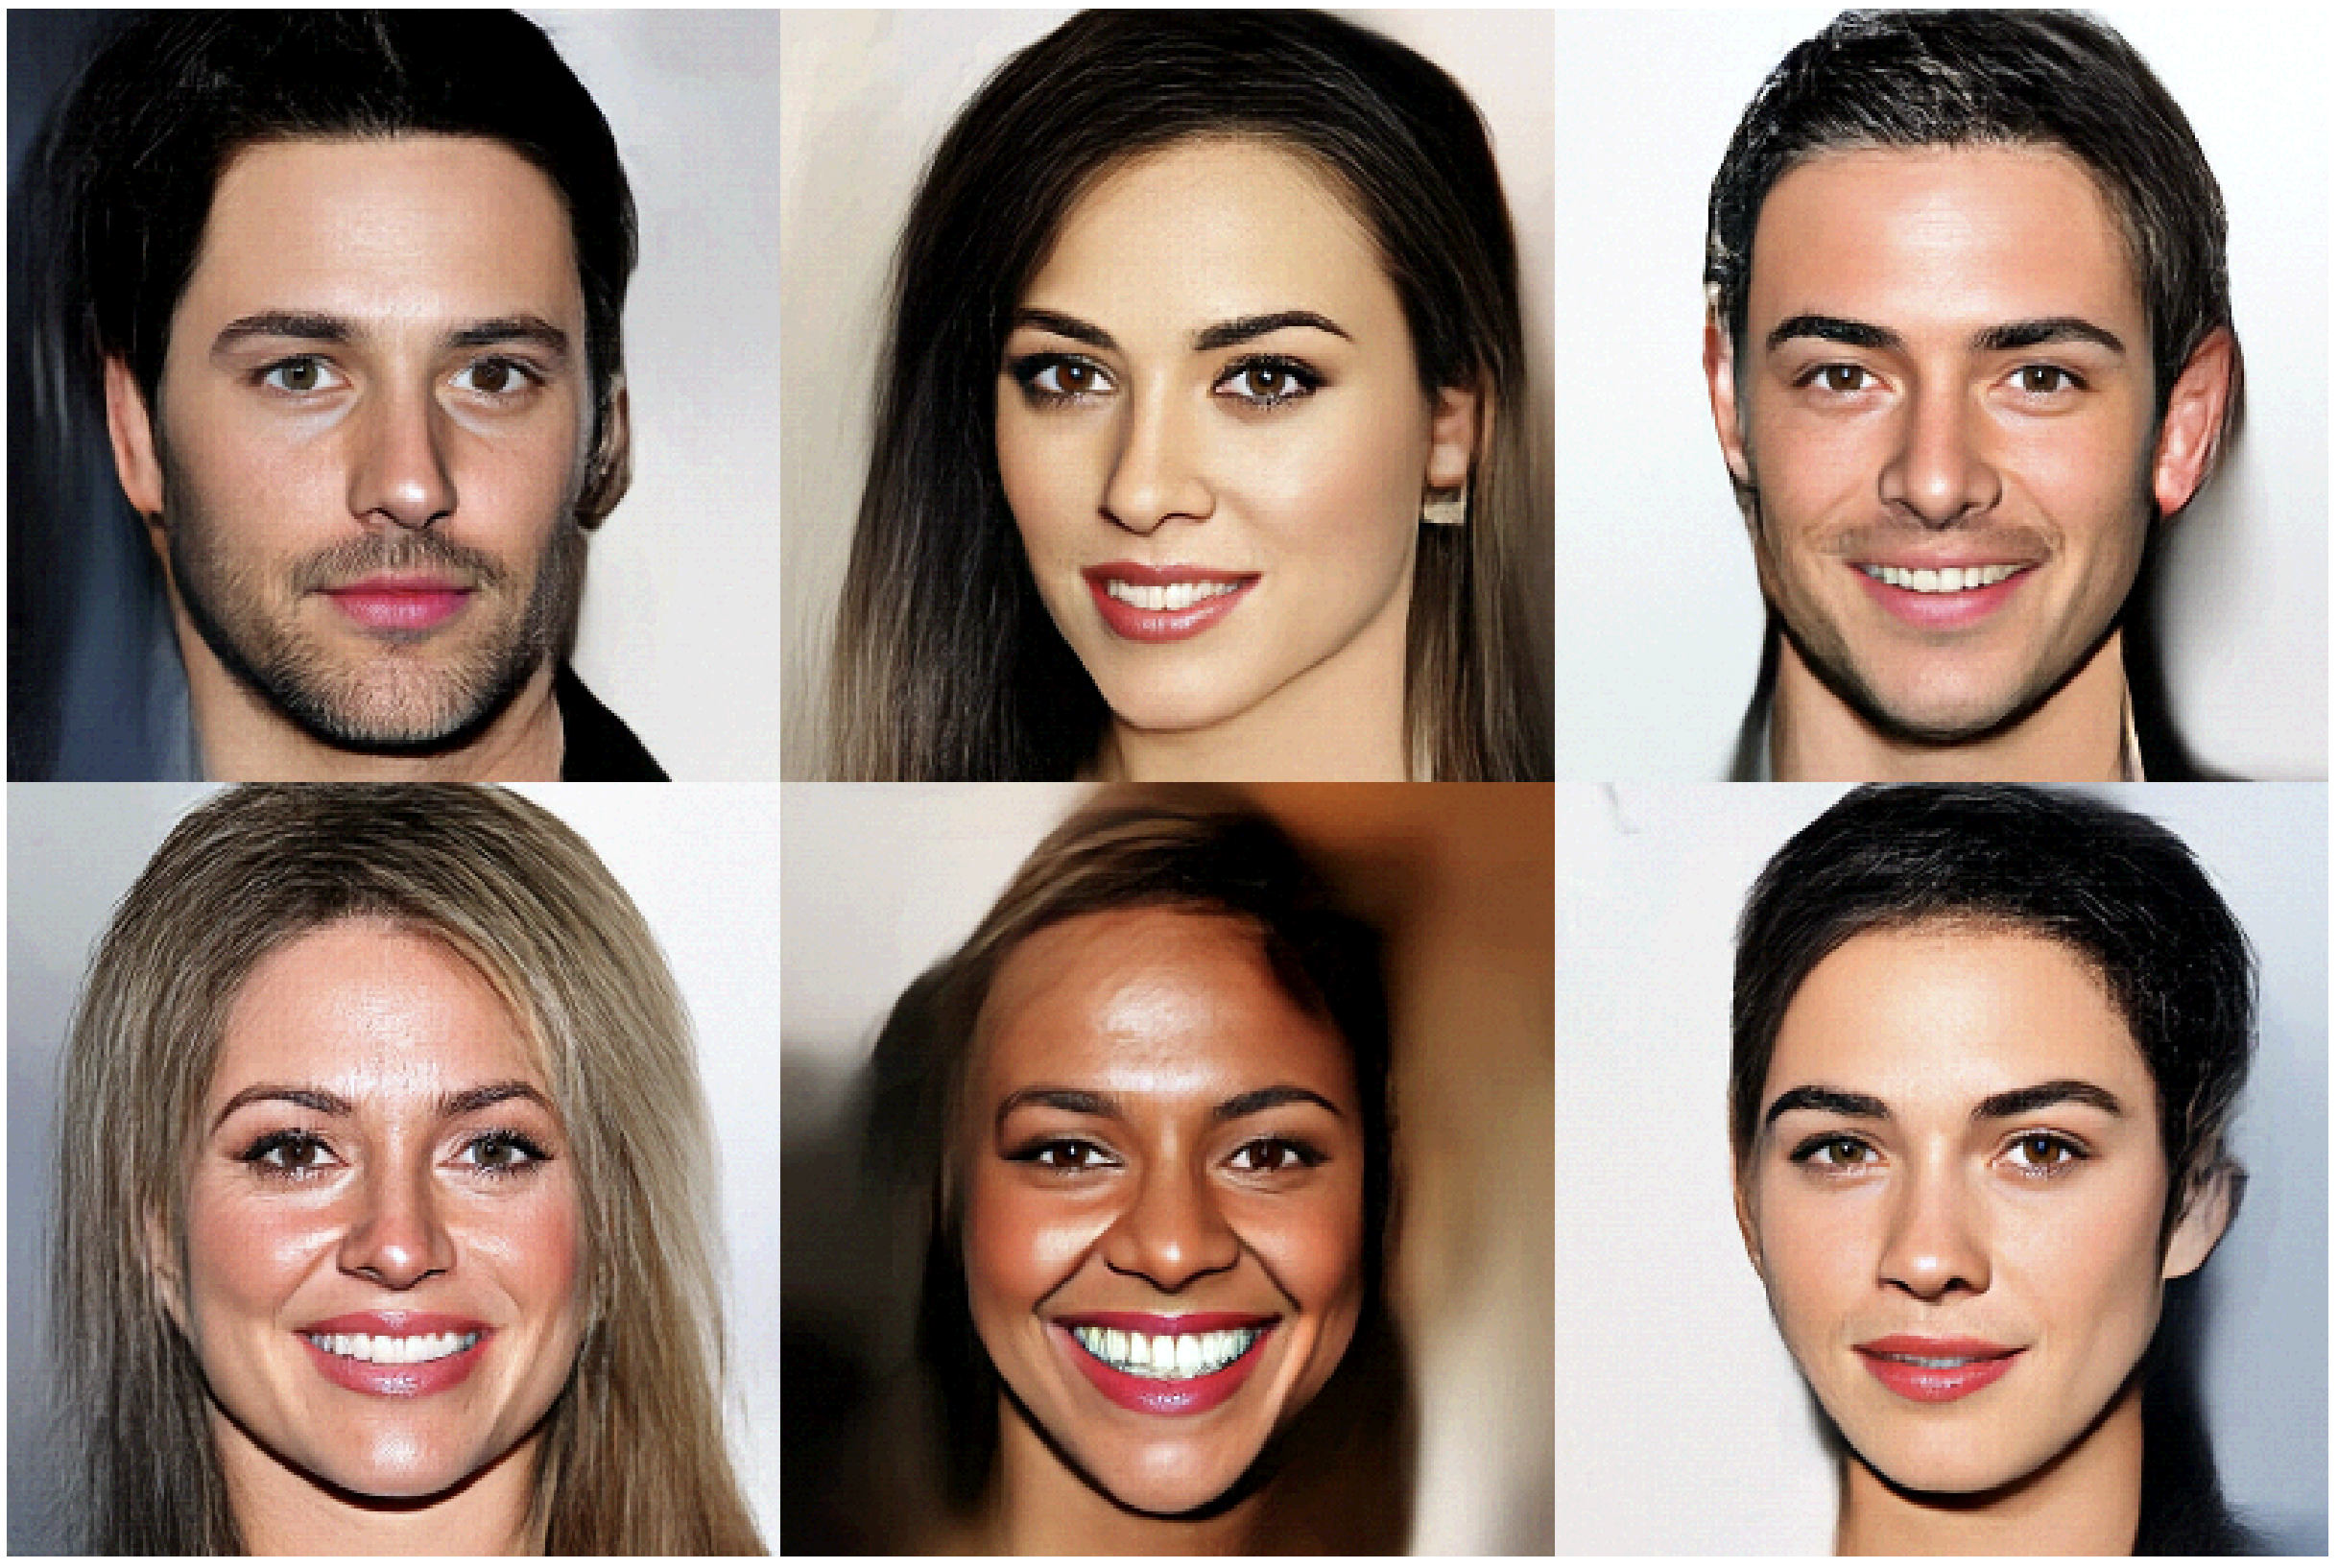
\includegraphics[width=0.9\linewidth]{figs/glow_faces.png}
	\end{figure}
\end{frame}
%=======
\begin{frame}{Summary}
	\begin{itemize}
		\item The change-of-variables theorem provides a method for computing a random variable's density under an invertible transformation.
		\vfill
		\item Normalizing flows transform a simple base distribution into a complex one via a sequence of invertible mappings, each with efficient Jacobian determinants.
		\vfill
		\item This enables exact likelihood computation, thanks to the change-of-variables formula.
		\vfill
		\item Linear NFs capture invertible matrices by using matrix decompositions.
		\vfill
		\item Gaussian autoregressive NFs are AR models with triangular Jacobians.
		\vfill
		\item The RealNVP coupling layer provides an efficient normalizing flow (a special case of AR NF), supporting fast inference and sampling.
	\end{itemize}
\end{frame}
\end{document}